
\documentclass[11pt,a4paper]{article}
\usepackage[utf8]{inputenc}
\usepackage[T1]{fontenc}
\usepackage{lmodern}
\usepackage{geometry}
\usepackage{hyperref}
\usepackage{longtable}
\usepackage{graphicx}
\geometry{margin=1in}

\title{Final Report: MSc Cybersecurity Admission Project}
\author{[Your Name]}
\date{May 3, 2025}

\begin{document}
\maketitle

\section*{GitHub Repository}
\noindent
\url{https://github.com/jafarizadeh/cybersup.git}

\section*{Executive Summary}
This report documents the three practical exercises completed as part of the MSc Cybersecurity admission process at Cybersup. The exercises cover core competencies in:
\begin{itemize}
  \item \textbf{Networking:} VLAN segmentation, DHCP, and inter–VLAN routing on Cisco devices.
  \item \textbf{System Administration:} Active Directory deployment and user/group automation via PowerShell.
  \item \textbf{DevOps/Containerization:} End–to–end WordPress deployment using Docker Compose.
\end{itemize}
All configurations, scripts, and supporting screenshots are available in the GitHub repository above.

\section*{Project Overview}
\begin{longtable}{|c|p{3cm}|p{5cm}|p{4cm}|}
    \hline
    \textbf{Exercise} & \textbf{Domain} & \textbf{Tools \& Technologies} & \textbf{Deliverables} \\ \hline
    1 & Networking & Cisco Packet Tracer, Cisco IOS & \texttt{.pkt} file, device configs, README \\ \hline
    2 & System Admin & Windows Server 2019/2022, PowerShell, CSV & PowerShell scripts, CSV, README \\ \hline
    3 & DevOps & Docker, Docker Compose, Nginx, PHP-FPM, MariaDB, WordPress & \texttt{docker-compose.yaml}, \texttt{nginx.conf}, README \\ \hline
\end{longtable}

\section{Exercise 1 – Networking with Cisco Packet Tracer}
\subsection{Objectives}
\begin{itemize}
  \item Design a small-scale enterprise network with four VLANs.
  \item Configure DHCP services on a Cisco 1941 router.
  \item Enable inter–VLAN routing and prepare for Internet connectivity.
\end{itemize}

\subsection{Equipment \& Topology}
\begin{itemize}
  \item \textbf{Router:} Cisco 1941
  \item \textbf{Switches:} 3 $\times$ Cisco (simulated in Packet Tracer)
  \item \textbf{Access Points:} 3 $\times$ PT-AC
  \item \textbf{Clients:} 6 desktop PCs, 3 laptops
  \item \textbf{IP Phones:} 3 $\times$ Cisco 7960
\end{itemize}

\paragraph{Logical Topology:}
\begin{figure}[h!]
    \centering
    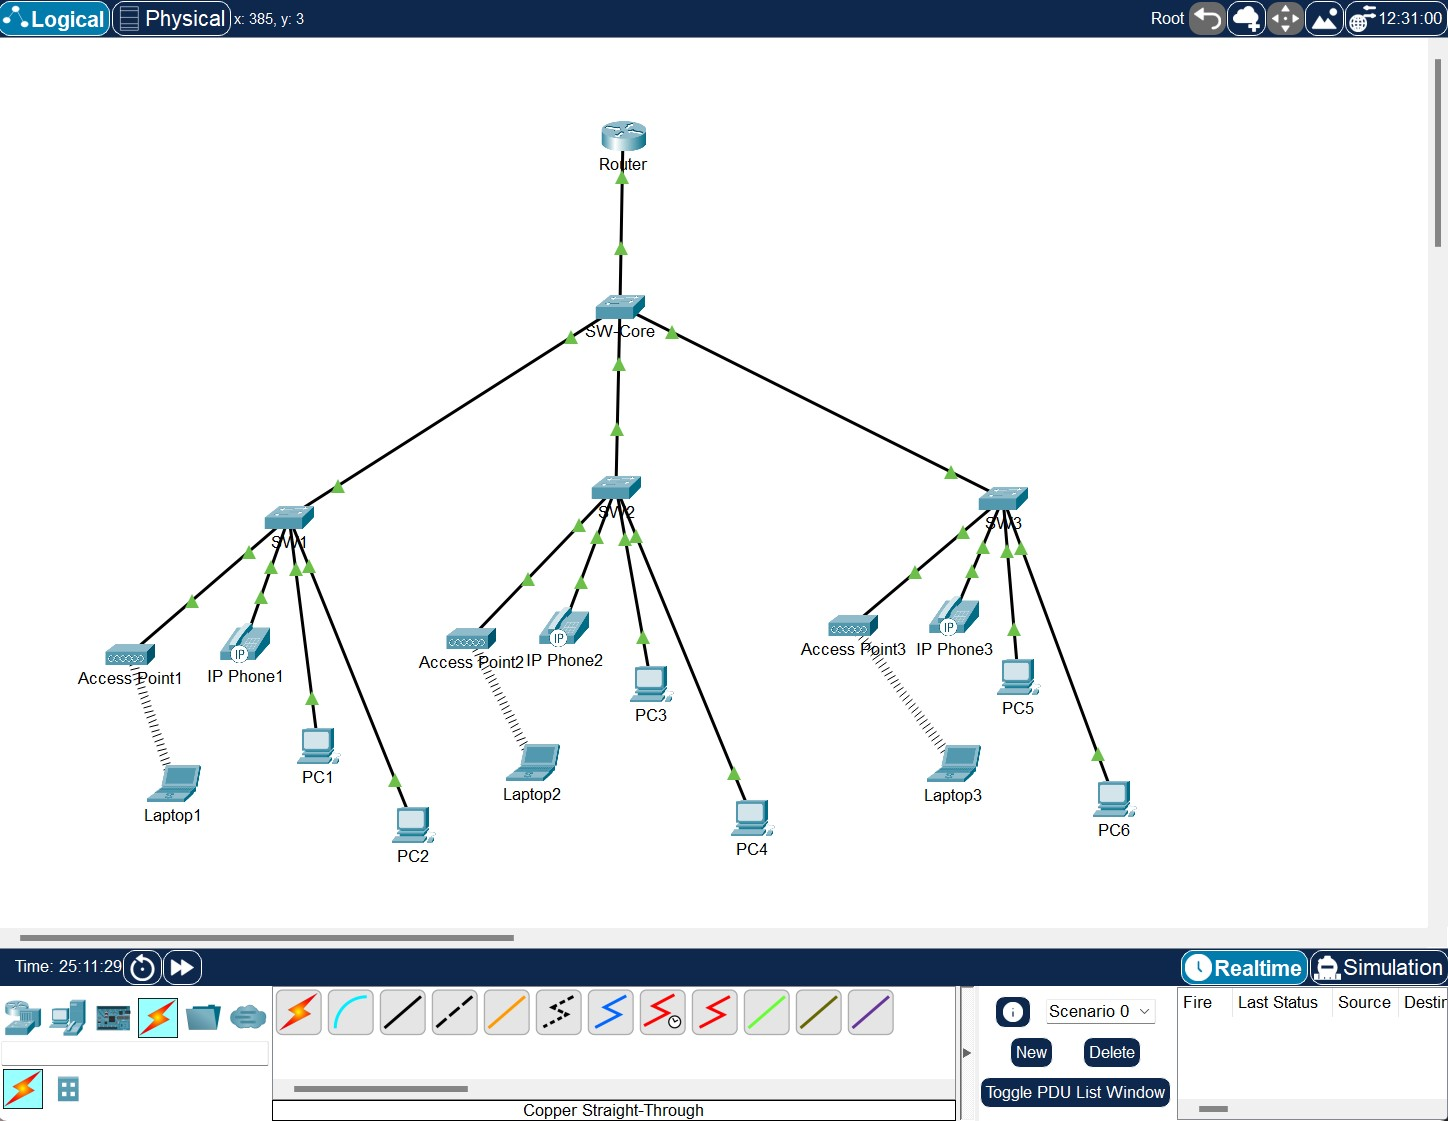
\includegraphics[width=\linewidth,height=0.75\textheight,keepaspectratio]{../Exercice 01 _ Packet Tracer/01.jpg}
    \caption{Logical Network Topology}
\end{figure}

\subsection{VLAN \& DHCP Configuration}
\begin{tabular}{|c|l|l|l|l|}
\hline
\textbf{VLAN ID} & \textbf{Name} & \textbf{Subnet} & \textbf{DHCP Range} & \textbf{Gateway} \\ \hline
1 & VoIP & 192.168.0.0/24 & .10–.50 & 192.168.0.1 \\ \hline
10 & WiFi & 192.168.10.0/24 & .10–.50 & 192.168.10.1 \\ \hline
20 & PC & 192.168.20.0/24 & .10–.50 & 192.168.20.1 \\ \hline
30 & Admin & 192.168.30.0/24 & .10–.50 & 192.168.30.1 \\ \hline
\end{tabular}

\subsection{Implementation Steps}
\begin{enumerate}
  \item Define VLANs and assign access/trunk ports on each switch.
  \item Configure sub-interfaces on the router with \texttt{encapsulation dot1Q} and DHCP pools.
  \item Connect devices, power on, and verify DHCP address allocation.
  \item Test inter–VLAN connectivity using ping.
\end{enumerate}

\subsection{Validation \& Results}
\begin{itemize}
  \item \textbf{Success:} All clients obtained IP addresses via DHCP.
  \item \textbf{Success:} Inter–VLAN routing validated by cross-VLAN pings.
  \item \textbf{Success:} Router reachability confirmed from each subnet.
\end{itemize}

\section{Exercise 2 – Active Directory Automation with PowerShell}
\subsection{Objectives}
\begin{itemize}
  \item Deploy an Active Directory domain \texttt{laplateforme.io} on Windows Server.
  \item Automate creation of 15 users and 9 groups from a CSV file.
  \item Enforce a strong password policy and require first-login password change.
\end{itemize}

\subsection{Environment Preparation}
\begin{itemize}
  \item OS: Windows Server 2019/2022
  \item Static IP (e.g., 192.168.1.100)
  \item Active Directory Domain Services (AD DS) role installed
\end{itemize}

\subsection{CSV Import Script}
\textbf{Sample CSV:}
\begin{verbatim}
nom,prénom,groupe1,groupe2,...
ALEXANDRE,MARCELLINE,Animation,
ARAGON,ISABELLE,Animation,
...
\end{verbatim}

\textbf{Scripts Provided:}
\begin{itemize}
  \item \texttt{AD-Setup.ps1}: Installs AD DS role and promotes server.
  \item \texttt{Create-UsersFromCSV.ps1}: Reads CSV, creates groups, users with default password \texttt{Azerty2025!}, enforces password change, and assigns groups.
\end{itemize}

\subsection{Password \& Security Policies}
\begin{verbatim}
Set-ADDefaultDomainPasswordPolicy `
  -Identity laplateforme.io `
  -ComplexityEnabled $true `
  -MinPasswordLength 8 `
  -MaxPasswordAge 42.00:00:00 `
  -LockoutThreshold 5 `
  -ReversibleEncryptionEnabled $false
\end{verbatim}

\subsection{Implementation Steps}
\begin{enumerate}
  \item Rename server and assign static IP.
  \item Install AD DS role and reboot.
  \item Promote to domain controller using \texttt{Install-ADDSForest}.
  \item Run \texttt{Create-UsersFromCSV.ps1} to import users and groups.
  \item Verify all accounts and memberships in Active Directory Users and Computers.
\end{enumerate}

\subsection{Validation \& Results}
\begin{itemize}
  \item Domain and DNS configured successfully.
  \item All 15 users and 9 groups created and correctly assigned.
  \item Password policy enforced and first-login password change required.
\end{itemize}

\section{Exercise 3 – Containerized WordPress with Docker Compose}
\subsection{Objectives}
\begin{itemize}
  \item Deploy a scalable WordPress site using Docker Compose.
  \item Use persistent volumes to retain data across container restarts.
\end{itemize}

\subsection{Service Architecture}
\begin{itemize}
  \item \textbf{mariadb:} Database service (volume \texttt{db\_data})
  \item \textbf{php-fpm:} PHP processor (volume \texttt{wordpress\_data})
  \item \textbf{wordpress:} CMS application
  \item \textbf{nginx:} Web server, port mapping 8080:80
\end{itemize}

\subsection{Configuration Files}
\textbf{docker-compose.yaml} and \texttt{nginx.conf} define services, volumes, networks, and Nginx settings (root, PHP upstream, static caching).

\subsection{Deployment Steps}
\begin{enumerate}
  \item Clone repository and navigate to \texttt{/exercise3/}.
  \item Run \texttt{docker-compose up -d}.
  \item Verify containers are running (\texttt{docker ps}).
  \item Access \url{http://localhost:8080} and complete WordPress setup.
\end{enumerate}

\subsection{Validation \& Results}
\begin{itemize}
  \item All containers started without errors.
  \item Data persisted after container restarts.
  \item WordPress installation wizard accessible and functional.
\end{itemize}

\section*{Challenges \& Solutions}
\begin{tabular}{|p{6cm}|p{8cm}|}
\hline
\textbf{Challenge} & \textbf{Solution} \\ \hline
VLAN misconfiguration on trunk ports & Reviewed and corrected \texttt{switchport trunk native vlan} settings \\ \hline
PowerShell errors during group creation & Added \texttt{Try/Catch} blocks with logging \\ \hline
Docker volume permission issues & Adjusted host folder ownership and permissions \\ \hline
\end{tabular}

\section*{Conclusion}
The admission project successfully demonstrates:
\begin{itemize}
  \item \textbf{Network Engineering:} VLAN design, DHCP, inter–VLAN routing on Cisco.
  \item \textbf{Systems Administration:} Automated AD deployment and user management via PowerShell.
  \item \textbf{DevOps:} Container orchestration with Docker Compose and Nginx.
\end{itemize}
For detailed configurations, scripts, and screenshots, please explore the subdirectories:
\begin{itemize}
  \item \texttt{/exercise1/}
  \item \texttt{/exercise2/}
  \item \texttt{/exercise3/}
\end{itemize}

\end{document}